\documentclass[simplex.tex]{subfiles}
% NO NEED TO INPUT PREAMBLES HERE
% packages are inherited; you can compile this on its own
\begin{document}
\subsection{Low-rank Assumption Discussion}
%As we noted above, if the graphs are distributed according to an SBM or an RDPG, the relative efficiency is approximately invariant to the number of graphs $M$ when $N$ is large.
%If on the other hand, the graphs are generated according to a full-rank independent edge model, then the relative efficiency can change more dramatically as $M$ changes. 
%The reason for this is because for larger $M$, more of the eigenvectors of $\bar{A}$ will begin to concentrate around the eigenvectors of the mean graph.
%This leads to the fact that the optimal embedding dimension for estimating the mean will increase, making $\bar{A}$ and the low-rank approximation at the optimal dimension closer together. 
%As a result, $\mathrm{RE}(\bar{A},\hat{P})$ will increase as $M$ increases for full-rank models.
%Indeed, for large $M$ we could have $\mathrm{RE}(\bar{A},\hat{P})\geq 1$ since we cannot guarantee that $\hat{P}$ will choose the optimal dimension.
%The lack of gaps in the eigenvalues of the mean graph makes dimension reduction quite dangerous.
%In an extreme case, the low-rank assumption will be mostly violated when all eigenvalues of the mean graph are almost equal. This leads to a certain type of structure, which is close to a constant times the identity matrix. However we don't see such structure in connectomoics. Now we check this before applying our estimator to the CoRR dataset.
%
%
%We first check if the dataset has the low-rank property. In Fig.~\ref{fig:screeplot}, we plot the eigenvalues of the mean graph of all 454 graphs (with diagonal augmentation) in decreasing algebraic order for three different atlases. For all three atlases, the eigenvalues first decrease dramatically and then stay around 0. In addition, we also plot the histograms in Fig.~\ref{fig:histogram}. From the figures we can see many eigenvalues are around zero, with a few large eigenvalues. So the information is mostly contained in the first few dimensions. Such quasi low-rank property could be used by $\hat{P}$ to improve $\bar{A}$.
%\begin{figure}[!htbp]
%\centering
%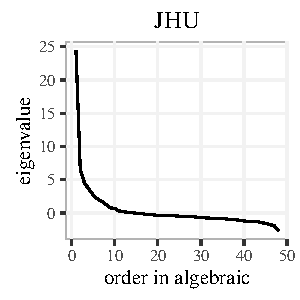
\includegraphics[height=.2\textheight]{../../figs/screeplot_JHU.pdf} 
%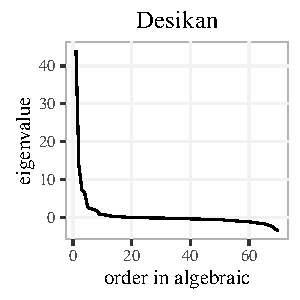
\includegraphics[height=.2\textheight]{../../figs/screeplot_desikan.pdf} 
%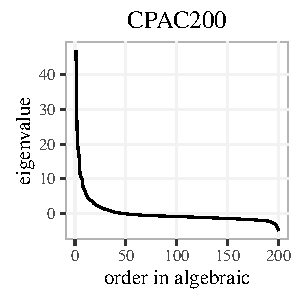
\includegraphics[height=.2\textheight]{../../figs/screeplot_CPAC200.pdf}
%\caption{{\bf Screeplot of the population mean.}
%These screeplots show the eigenvalues of the mean graph of all 454 graphs with diagonal augmentation in decreasing algebraic order for three atlases. Many eigenvalues are around zero, which lead to a quasi low-rank structure.
%}
%\label{fig:screeplot}
%\end{figure}
%
%\begin{figure}[!htbp]
%\centering
%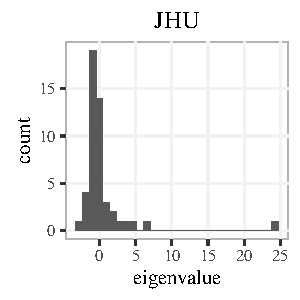
\includegraphics[height=.2\textheight]{../../figs/hist_JHU.pdf} 
%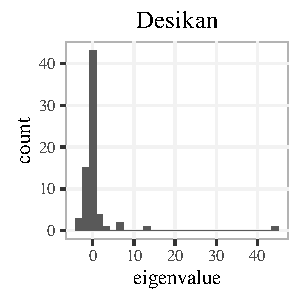
\includegraphics[height=.2\textheight]{../../figs/hist_desikan.pdf} 
%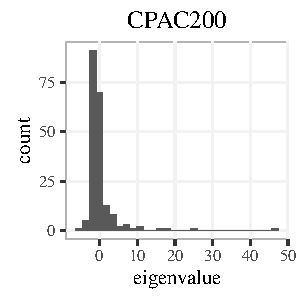
\includegraphics[height=.2\textheight]{../../figs/hist_CPAC200.pdf}
%\caption{{\bf Histogram of the population mean.}
%These figures show the histograms of the eigenvalues of the mean graph of all 454 graphs with diagonal augmentation. Many eigenvalues are around zero, which lead to a quasi low-rank structure.
%}
%\label{fig:histogram}
%\end{figure}
%
%
%
%
%\subsubsection{Interpretability of the Latent Positions}
%We also note that low-rank methods can often be more easily interpreted.
%By representing a low-rank matrix in terms of the latent position, where each vertex is represented as a vector in $\Re^d$ and the entries of the matrix are given by the inner products of these vectors, one can analyze and visualize the geometry of these vectors in order to interpret how each vertex is behaving in the context of the larger graph. 
%Now we take the CoRR dataset experiment as an example and consider the same sample of size $M=5$ based on the Desikan atlas. Our estimator $\hat{P}$ is based on the estimated latent positions $\hat{X} \in \mathbb{R}^{N\times d}$, where $N=70$ is the number of vertices and $d=11$ is the dimension selected by the Zhu and Ghodsi's method. Now we plot the heat map of $\hat{X}$ in Fig.~\ref{fig:eigenvector}, with each row to be the estimated latent position for the corresponding vertex. From the second column, we can see a clear distinction of the left and right hemisphere as conveyed in the second dimension. To have a more direct understanding of how they distinguish the two hemispheres, we color the brain using the 2nd dimension of $\hat{X}$ as in Fig.~\ref{fig:eigenvector_brain}. Additionally, such a representation allows the use of techniques from multivariate analysis to further study the estimated population mean.
%
%
%\begin{figure}[!htbp]
%\centering
%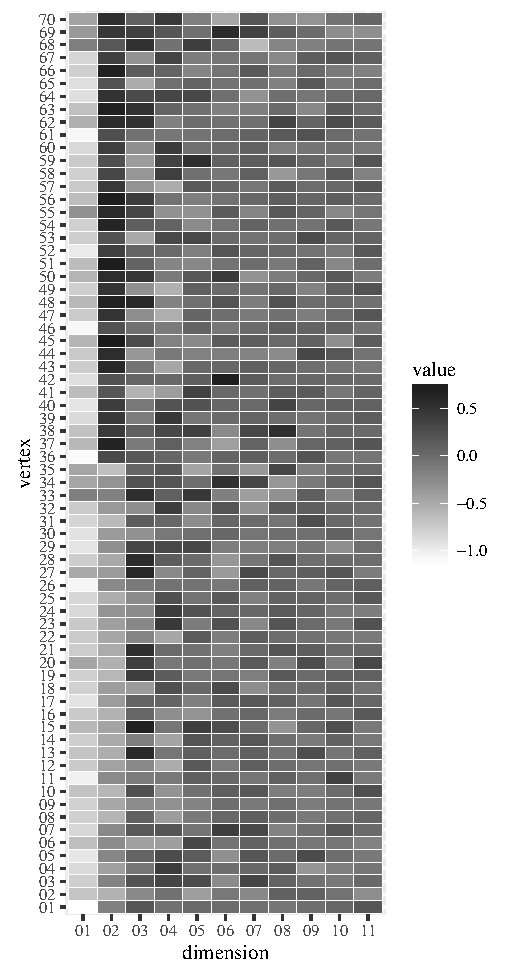
\includegraphics[width=.7\textwidth]{../../figs/eigenvector.pdf}
%\caption{{\bf Heat map of $\hat{X}$.}
%Heat map of $\hat{X}$ with each row to be the estimated latent position for the corresponding vertex. From the second column, we can see a clear distinction of the left and right hemisphere as conveyed in the second dimension.}
%\label{fig:eigenvector}
%\end{figure}
%
%\begin{figure}[!htbp]
%\begin{center}
%  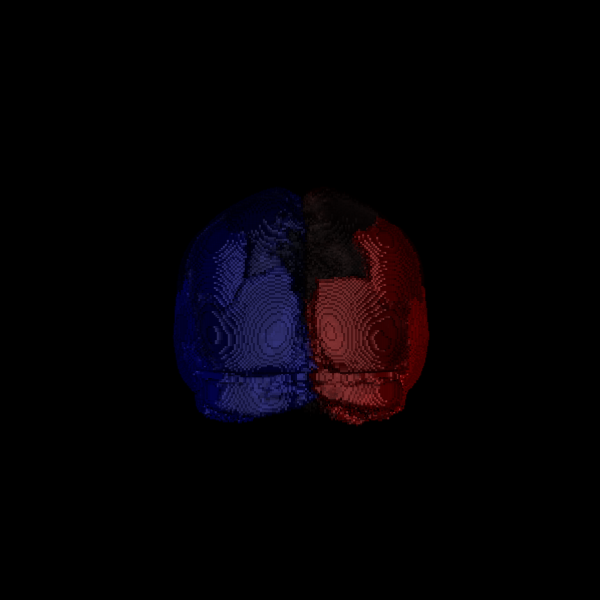
\includegraphics[height=.4\linewidth]{../../figs/desikan2.png}\hspace{-50pt}
%  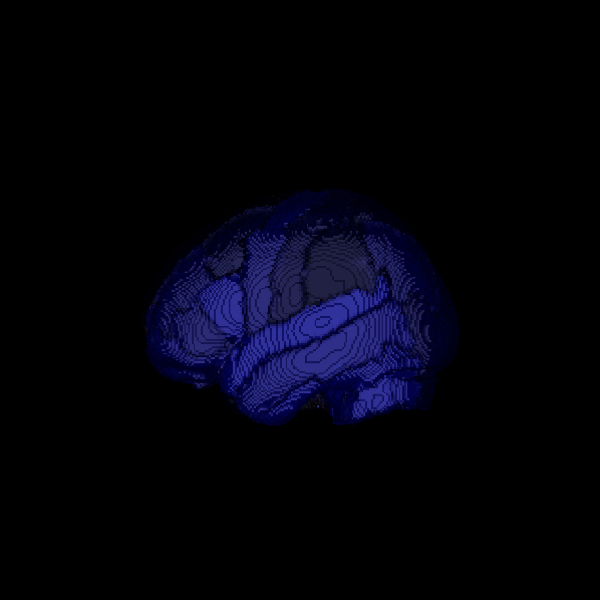
\includegraphics[height=.4\linewidth]{../../figs/desikan0.png}\hspace{-50pt}
%  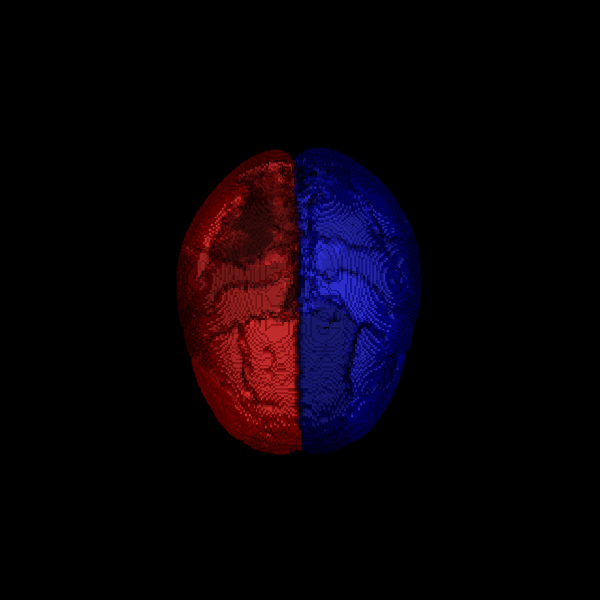
\includegraphics[height=.4\linewidth]{../../figs/desikan.png}
%\end{center}
%\caption{{\bf Brain colored by the 2nd dimension of $\hat{X}$.}
%We plot the brain using the 2nd dimension of $\hat{X}$. From the figure, we can see a clear distinction of the left and right hemisphere as conveyed in the second dimension.}
%\label{fig:eigenvector_brain}
%\end{figure}
%
%
%
\end{document}
